\documentclass[11pt, a4paper]{article}

% --- 宏包准备 ---
\usepackage[utf8]{inputenc}
\usepackage{graphicx} 
\usepackage{booktabs} 
\usepackage{amsmath}  
\usepackage{geometry} 
\geometry{margin=1in}
\usepackage{hyperref} 

% --- 标题信息 ---
\title{Clinical Mortality Prediction in Heart Failure Patients: A Comparative Study of Machine Learning and Neural Networks}
\author{Tongyang Zou}
\date{\today}

\begin{document}

\maketitle

\begin{abstract}
Heart failure is a leading cause of cardiovascular mortality worldwide. This study leverages a dataset of 299 clinical records to develop a predictive model for patient survival. We performed data preprocessing, feature engineering, and compared multiple algorithms including Logistic Regression, Random Forest, and Multi-Layer Perceptron (MLP). Our results show that follow-up time, serum creatinine, and ejection fraction are the most critical predictors, with the XGBoost model achieving a superior AUC compared to traditional methods.
\end{abstract}

\section{Introduction}
Predicting the risk of death in heart failure patients is crucial for clinical decision-making. Traditional scoring systems often fail to capture non-linear relationships between bio-markers. This paper aims to utilize the Heart Failure Clinical Records dataset to build a robust predictive pipeline.

\section{Methods}
This analytical pipeline follows the methodology established by Chicco and Jurman \cite{chicco2020machine}, prioritizing key clinical features for mortality prediction.
% --- 图 1：AI 概念工作流程图 ---
\begin{figure}[htbp]
    \centering
    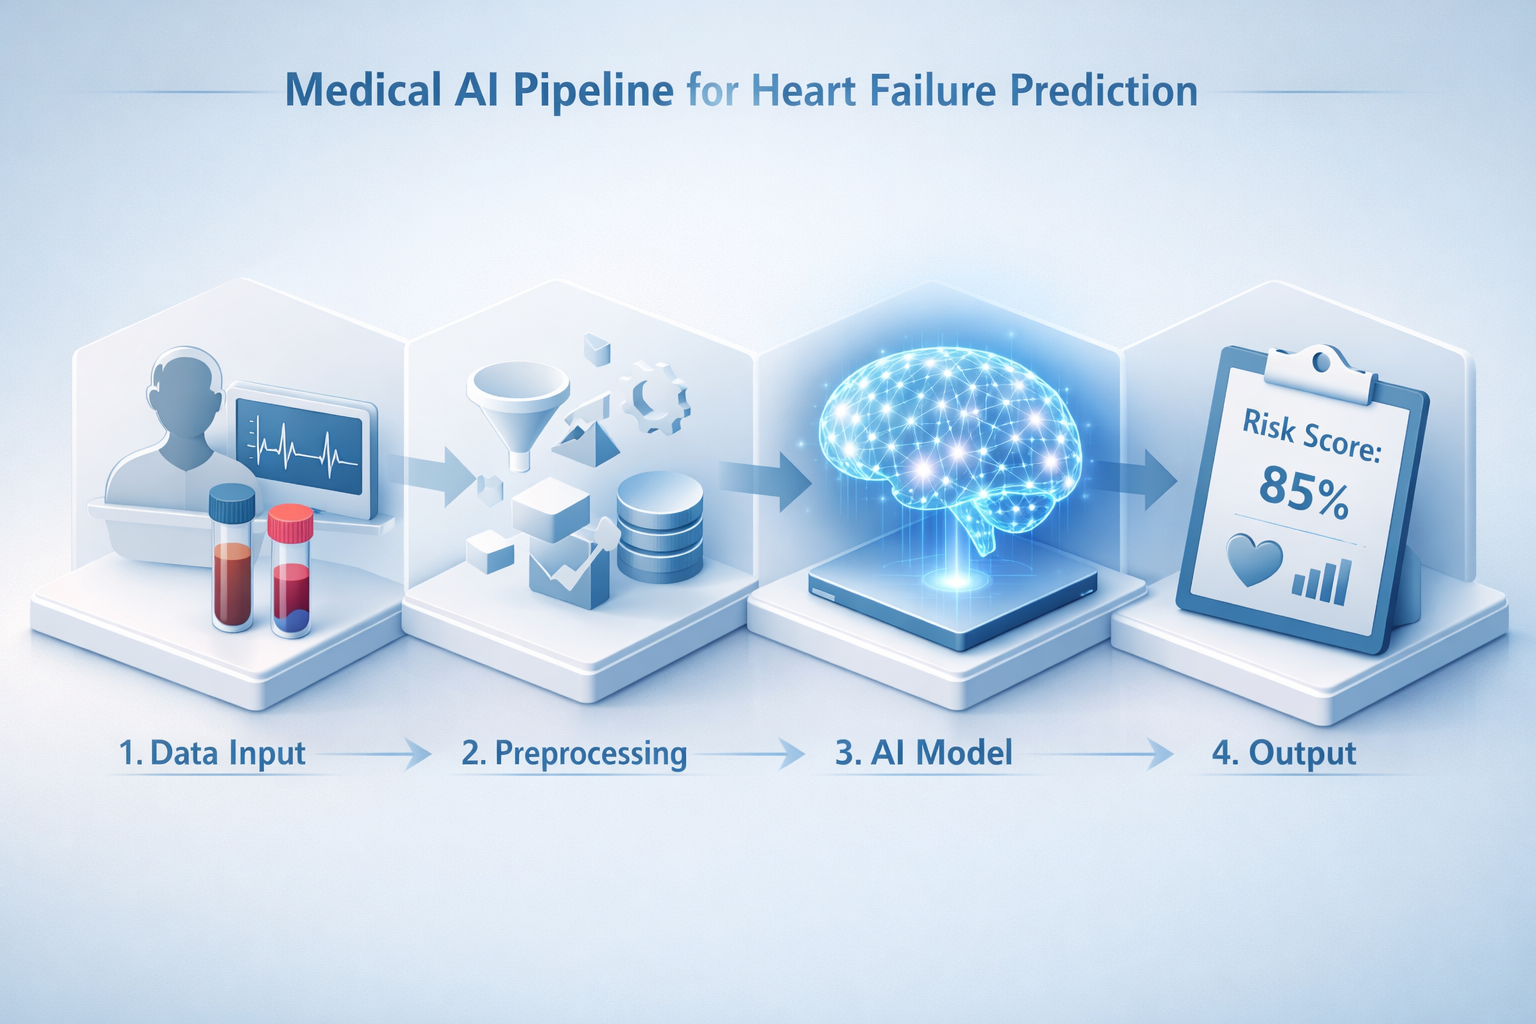
\includegraphics[width=0.7\textwidth]{workflow.png} 
    \caption{The proposed AI-driven clinical decision support framework for heart failure mortality prediction.}
    \label{fig:workflow}
\end{figure}

\subsection{Data Preprocessing}
The dataset contains 13 features. We handled outliers using clipping (1st and 99th percentiles) and applied Z-score standardization:
$$ z = \frac{x - \mu}{\sigma} $$
where $\mu$ is the mean and $\sigma$ is the standard deviation. This ensures that features like \textit{platelets} and \textit{serum creatinine} are on the same numerical scale, allowing models like Logistic Regression and MLP to converge efficiently.

\section{Results and Discussion}

\subsection{Exploratory Data Analysis}
Before modeling, we evaluated the correlation between clinical features. As shown in Figure \ref{fig:heatmap}, several features exhibit significant associations with the mortality event.

% --- 图 2：相关性热力图 (Figure_1.png) ---
\begin{figure}[htbp]
    \centering
    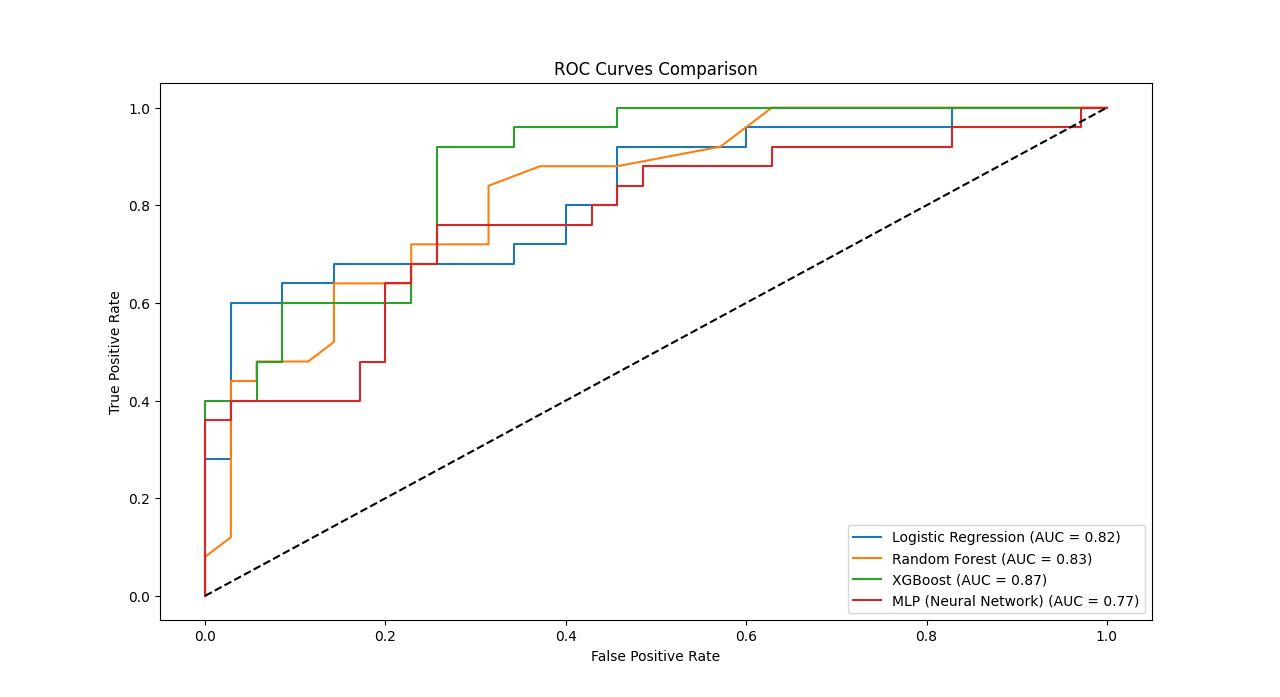
\includegraphics[width=0.6\textwidth]{Figure_1.png} 
    \caption{Correlation heatmap of clinical features and the target variable (DEATH\_EVENT).}
    \label{fig:heatmap}
\end{figure}

\subsection{Feature Importance}
Using a Random Forest classifier, we identified the top predictors. Figure \ref{fig:importance} illustrates that \textit{time} (follow-up period), \textit{serum\_creatinine}, and \textit{ejection\_fraction} dominate the model's decision-making process, aligning with clinical observations.

% --- 图 3：特征重要性 (Figure_2.png) ---
\begin{figure}[htbp]
    \centering
    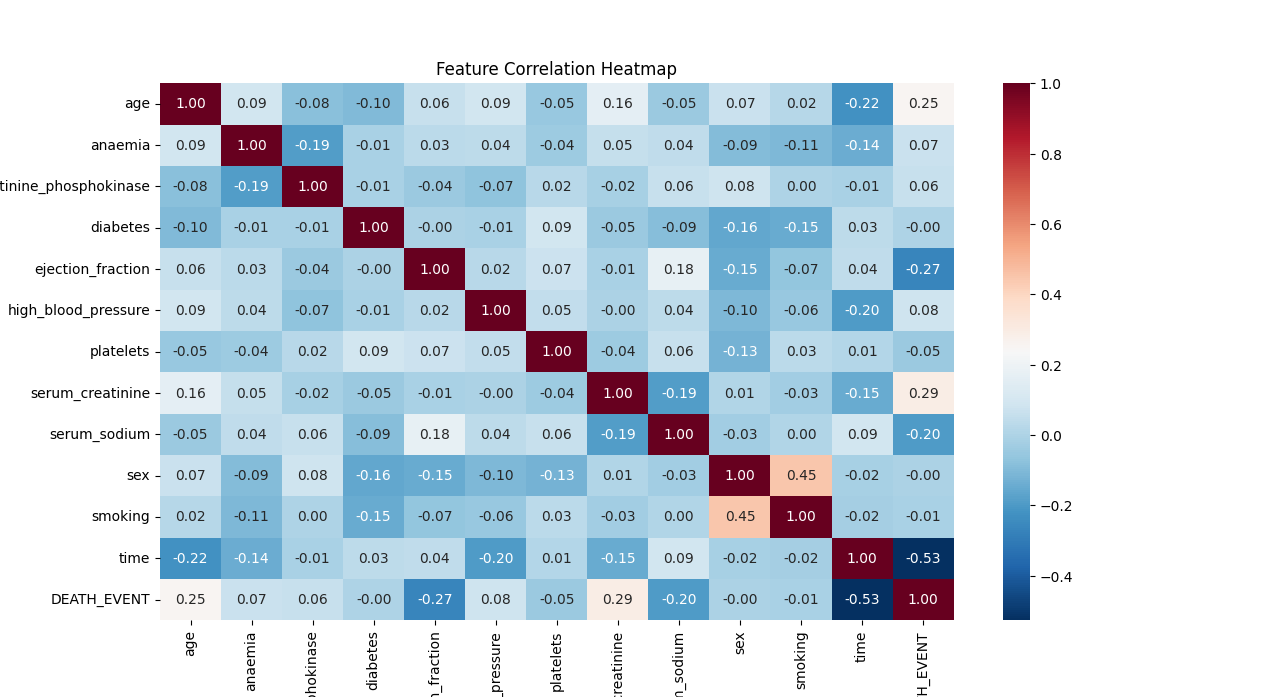
\includegraphics[width=0.6\textwidth]{Figure_2.png}
    \caption{Feature importance ranking derived from the tree-based ensemble model.}
    \label{fig:importance}
\end{figure}

\subsection{Model Performance}
We evaluated models using the $F_1$ score, defined as the harmonic mean of precision and recall:
$$ F_1 = 2 \cdot \frac{\text{precision} \cdot \text{recall}}{\text{precision} + \text{recall}} $$

The performance metrics obtained from our experimental code are summarized in Table \ref{tab:results}.

\begin{table}[htbp]
    \centering
    \caption{Comparison of machine learning model performance}
    \label{tab:results}
    \begin{tabular}{lcccc}
        \toprule
        Model & Accuracy & Precision & Recall & AUC \\
        \midrule
        Logistic Regression  & \textbf{0.80} & \textbf{0.93} & 0.56 & 0.82 \\
        Random Forest        & 0.75 & 0.86 & 0.48 & 0.83 \\
        XGBoost              & 0.78 & 0.83 & \textbf{0.60} & \textbf{0.87} \\
        MLP (Neural Network) & 0.67 & 0.63 & 0.48 & 0.77 \\
        \bottomrule
    \end{tabular}
\end{table}

\subsection{ROC Analysis}
The Receiver Operating Characteristic (ROC) curves in Figure \ref{fig:roc} demonstrate the superior discriminative power of ensemble methods (XGBoost and Random Forest) over the Multi-Layer Perceptron and baseline Logistic Regression.

% --- 图 4：ROC 曲线 (Figure_3.png) ---
\begin{figure}[htbp]
    \centering
    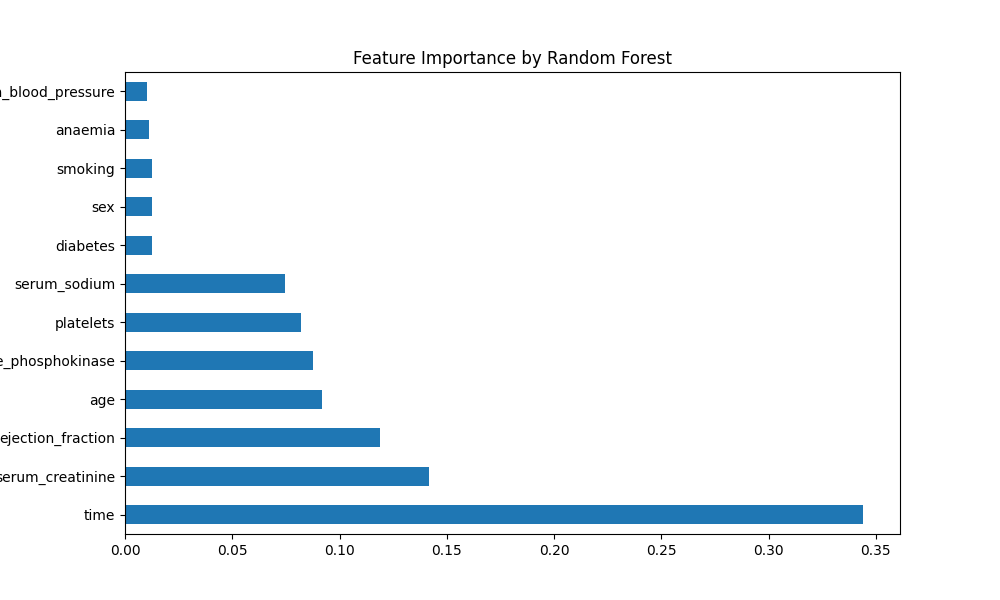
\includegraphics[width=0.6\textwidth]{Figure_3.png}
    \caption{ROC curves comparison across four different predictive models.}
    \label{fig:roc}
\end{figure}

\section{Conclusion}
This study proves that machine learning, especially gradient boosting algorithms like XGBoost, can effectively predict mortality in heart failure patients using routine clinical data. The integration of such models into clinical workflows could provide valuable early warnings for high-risk patients.

\bibliographystyle{plain} % 规定引用格式为标准数字格式
\bibliography{references} % 链接到刚才创建的 references.bib 文件

\end{document}